\documentclass[PI,LAB]{HSEUniversity}
% Возможные опции: KR или VKR; PI или BI
\usepackage{svg}
\usepackage{listings}

\title{Организация паттернов проектирования. Структурный паттерн Заместитель}
\author{Виноградов Никита Андреевич}
\supervisor{к.т.н., доцент кафедры Информационных технологий в бизнесе НИУ ВШЭ-Пермь}{А.В.~Кычкин}

\Year{2020}


% Ссылка на файл с описание библиографии
\bibliography{library.bib}

%%%%%%%%%%%%%%%%%%%%%%%%%%%%%%%%
%%% ТЕКСТ РАБОТЫ %%%%%%%%%%%%%%%
\begin{document}

    % Обязательные элементы оформления: заголовочный слайд, аннотация, оглавление
    \maketitle



    \chapter{Заместитель}
      это структурный паттерн проектирования, который позволяет подставлять вместо реальных объектов специальные объекты-заменители. Эти объекты перехватывают вызовы к оригинальному объекту, позволяя сделать что-то до или после передачи вызова оригиналу.
    \section{Назначение}
    Заместитель предлагает создать новый класс-дублёр, имеющий тот же интерфейс, что и оригинальный служебный объект. При получении запроса от клиента объект-заместитель сам бы создавал экземпляр служебного объекта и переадресовывал бы ему всю реальную работу.
    \section{Структура}

    \begin{FIGURE}[h]{Структура классов паттерна Заместитель\label{fig:example-figure}}
       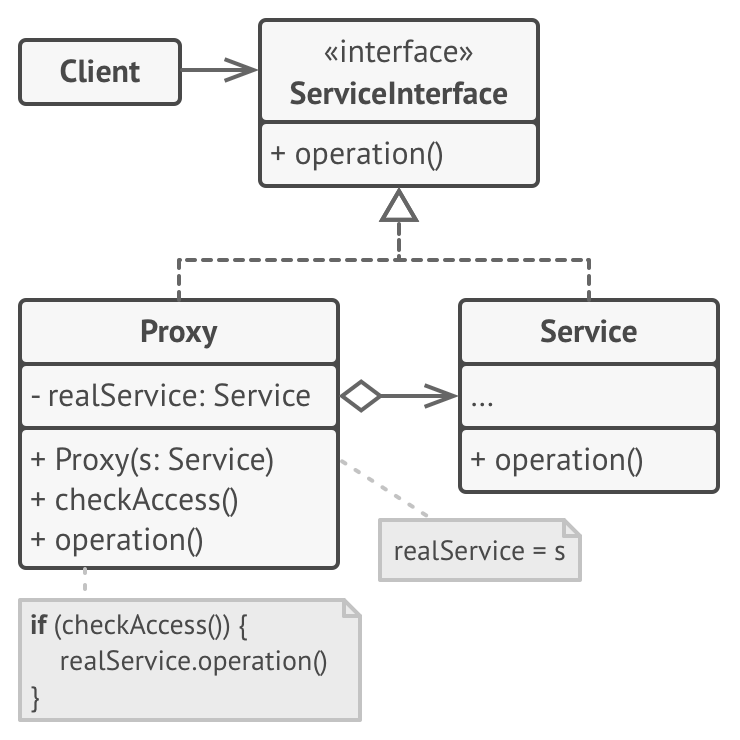
\includegraphics[width=0.4\textwidth]{../out/diagrams/structure-ru}
    \end{FIGURE}

    \textbf{Участники:}
   		\begin{itemize}
   			\item \emph{Client} - класс который вызывает методы компонента
   		\item \emph{Service Interface} - определяет общий интерфейс для сервиса и заместителя
   		\item \emph{Proxy} -  хранит ссылку на объект сервиса ,  передаёт вызовы вложенному сервису.
   		\item \emph{Service} - Класс содержащий бизнес-логику проекта
   		\end{itemize}

 \begin{FIGURE}[h]{Диаграмма последовательности паттерна Заместитель\label{fig:example-figure}}
	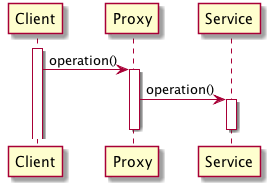
\includegraphics[width=0.4\textwidth]{../out/diagrams/default/compactors}
\end{FIGURE}
    \section{Способ применения}
    Данный паттерн необходим когда необходимо перехватывать операции в системе для валидации данных или придания дополнительной логики.
    \chapter{Реализация паттернов}

    \section{Диаграмма классов}
     \begin{FIGURE}[h]{Диаграмма классов паттерна Компоновщик\label{fig:example-figure}}
    	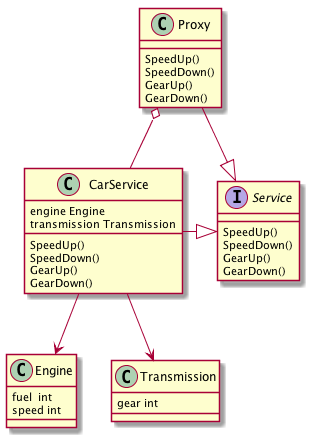
\includegraphics[width=0.4\textwidth]{../out/diagrams/builder/compactor}
    \end{FIGURE}
	\emph{Участники:}
	\begin{itemize}
	
		\item \emph{Client} - класс который вызывает методы компонента
	\item \emph{Service Interface} - определяет общий интерфейс для сервиса и заместителя
	\item \emph{Proxy} -  хранит ссылку на объект сервиса ,  передаёт вызовы вложенному сервису.
	\item \emph{CarService} - Сервис вызывающий функции в элементах автомобиля
	\end{itemize}
\pagebreak
    \section{Диаграмма последовательности }
  
	\begin{FIGURE}[h]{Диаграмма последовательности паттерна Компоновщик\label{fig:example-figure}}
		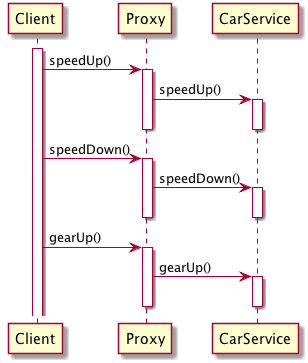
\includegraphics[width=0.3\textwidth]{../out/diagrams/builder-seq/compactor-seq}
	\end{FIGURE}


   


    \section{Код программы}
    \lstset{extendedchars=\true}
    \begin{lstlisting}[language=Go]
    package car
    
    import (
    "container/list"
    "reflect"
    )
    
    func TypeFlex(v interface{}) string {
    return reflect.TypeOf(v).String()
    }
    
    type Car struct {
    Container *list.List
    }
    
    func (e Car) Print(num int) {
    for e := e.Container.Front(); e != nil; e = e.Next() {
    
    switch str := e.Value.(type) {
    case CartPart:
    println(TypeFlex(e.Value))
    
    
    str.Print(num + 1)
    break
    }
    }
    }
    func (e Car) AddPart(part interface{}) {
    
    e.Container.PushBack(part)
    println(e.Container.Len())
    }
    func (e Car) RemovePart(part *interface{}) {
    el := list.Element{Value: part}
    e.Container.Remove(&el)
    }
    
    type CartPart interface {
    Print(num int)
    }
    package car
    
    import "container/list"
    
    //Демпфирующий
    //Стабилизатор
    //Стойка
    //Рычаг
    //Пружина
    //Амортизатор
    
    type Damping struct {
    }
    type Stabilizer struct {
    }
    type Rack struct {
    }
    type Lever struct {
    }
    type Spring struct {
    }
    type Absorber struct {
    }
    type Suspenstion struct {
    Container *list.List
    }
    
    func (e Suspenstion) Print(num int) {
    for e := e.Container.Front(); e != nil; e = e.Next() {
    for i := 0; i < num; i++ {
    print("-")
    }
    println(TypeFlex(e.Value))
    }
    }
    
    func (e Suspenstion) AddPart(part interface{}) {
    e.Container.PushBack(part)
    
    }
    func (e Suspenstion) RemovePart(part *interface{}) {
    el := list.Element{Value: part}
    e.Container.Remove(&el)
    }
    
    func NewSuspenstion() Suspenstion {
    return Suspenstion{Container: list.New()}
    }
    package car
    
    //блока цилиндров с картером,
    //
    //- головки блока цилиндров,
    //
    //- поддона картера двигателя,
    //
    //- поршней с кольцами и пальцами,
    //
    //- шатунов,
    //
    //- коленчатого вала,
    //
    //- маховика.
    import (
    "container/list"
    )
    
    type Engine struct {
    Container *list.List
    }
    
    func (e Engine) Print(num int) {
    for e := e.Container.Front(); e != nil; e = e.Next() {
    for i := 0; i < num; i++ {
    print("-")
    }
    println(TypeFlex(e.Value))
    }
    }
    
    type CylinderBlock struct {
    }
    type Sump struct {
    }
    type Crankshaft struct {
    }
    type Rod struct {
    }
    
    func (e Engine) AddPart(part interface{}) {
    e.Container.PushBack(part)
    }
    func (e Engine) RemovePart(part *interface{}) {
    el := list.Element{Value: part}
    e.Container.Remove(&el)
    }
    
    type EnginePart struct {
    }
    
    \end{lstlisting}

\end{document}
